\documentclass{article}
\usepackage[margin=2cm]{geometry}

\input{./basic-tex-config/preamble.tex}

\graphicspath{{./images/}}

\title{ЛАБОЛАТОРНАЯ РАБОТА ПО КУРСУ\\ <<КВАНТОВЫЙ КОМПЬЮТЕР>>\\
Двухкубитовые квантовые схемы}
\date{Санкт-Петербург, 2017}
\author{Плотников Антон, А4101}

\begin{document}

\maketitle
\newpage

\section{Цель работы}
Изучение работы алгоритма Гровера.

\section{Задачи}

\begin{enumerate}
  \item	Определить номер элемента который ищется в базе.
  \item	Определить количество итераций необходимо в алгоритме для получения
    вероятности верного ответа близко к 1.
  \item	Найти зависимость количества итераций от количества элементов в базе.
  \item	Сравнить предыдущий результат с самым эффективным классическим алгоритмом (перебор).
  \item	Объяснить, почему при дальнейшем увеличении числа итераций эффективность падает.
\end{enumerate}

\section{Ход работы}

Количество кубитов $n = 4$, число элементов в базе $N = 2^n = 16$

Номер элемента который ищется в базе --- 3.

\begin{figure}[H]
  \centering
  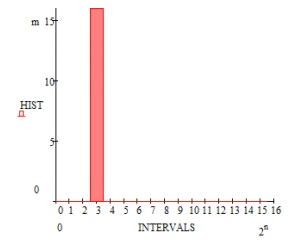
\includegraphics[width=0.6\textwidth]{graf_4_1}
  \caption{Гистограмма работы алгоритма Гровера ($R=3$)}\label{fig:41}
\end{figure}

Количество итераций необходимых для того чтобы ответ был с высокой вероятности
для случая 4 кубитов, равен 3


\begin{figure}[H]
  \centering
  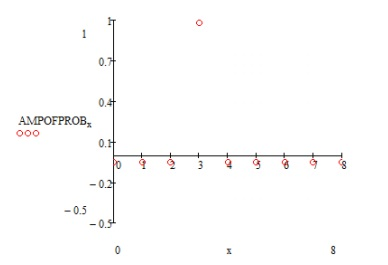
\includegraphics[width=0.6\textwidth]{graf_4_2}
  \caption{Амплитуды вероятностей ($R=3$)}\label{fig:42}
\end{figure}

Верхняя оценка числа итераций равна ($M$ --- количество решений удовлетворяющих
критерию поиска): 
\begin{equation}
  R \leqslant \left[\frac{\pi}{4} \sqrt{\frac{N}{M}}\right]
\end{equation}

В нашем случае $M = 1$ и выражение принимает вид:
\begin{equation}
  R \leqslant \left[\frac{\pi}{4} \sqrt{N}\right]
\end{equation}

Эффективность работы алгоритма Гровера $O(\sqrt{N})$, в то время когда
классический алгоритм поиска требует $O(N)$ операций. Как мы видим алгоритм
Гровера позволяет получить квадратичное улучшение в задаче поиска.

\begin{figure}[H]
  \centering
  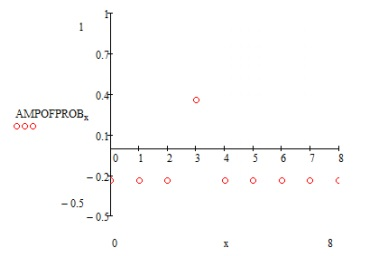
\includegraphics[width=0.6\textwidth]{graf_4_3}
  \caption{Амплитуды вероятностей ($R=5$)}\label{fig:43}
\end{figure}

Суть алгоритма заключается в изменении целевого состояния за счет  убывания
амплитуды всех остальных состояний. В том случае когда мы совершаем
дополнительные итерации амплитуды всех остальных состояний становятся
отрицательными, а следовательно и среднее значение также отрицательно, а так
как амплитуда искомого элемента откладывается от среднего значения, то в
результате мы получаем уменьшение амплитуды искомого элемента
(рис.~\ref{fig:43}).

\section{Вывод}

В ходе выполнения работы изучили работу квантового алгоритма поиска (алгоритм
Гровера). Определили количество итераций необходимых для определения искомого
элемента с вероятностью близкой к единице $R = 3$, во общем виде зависимость
итераций от количества элементов в базе выражается $R \leqslant
\left[\frac{\pi}{4} \sqrt{\frac{N}{M}}\right]$. Алгоритм Гровера позволяет
получить квадратичное улучшение по сравнению с классическим алгоритмом поиска.
Увеличение количества итераций ведет к падению эффективности, что вызвано
изменением знака среднего значения амплитуд.

\end{document} 
